% !TEX root = _individual/flatland.tex

%%%%%%%%%%%%%%%%%%%%%%%%%%%%%%%%%%%%%%%%%%%%%%%%%%%%%%%%%%%%%%%%%%%%%%%%%%%%%%%%
\chapter{Flatland Geometry}\label{chap:flatland}

``Flatland'' is a fictional two-dimensional universe in which particles are
constrained to exist and
travel in a 2-D plane \cite{Asa2008}. Because the flatland phase space is
$(x,y,\omega)$ with \emph{one} angular variable (the azimuthal~$\omega$),
rather than the
standard 2-D $(x,y,\mu,\omega)$ with \emph{two} angular variables (the
polar cosine~$\mu$ and the azimuthal~$\omega$),
flatland is a computationally simpler testing ground that retains the
complexity of multidimensional geometry. For this reason, flatland has recently
been used in the development and testing of multi-D transport methods, including
the new anisotropic diffusion method \cite{Lar2009c,Joh2011,Tra2011}.

Previous work has shown that the 3-D diffusion coefficient
$\frac{1}{3\sigma}$ differs from the flatland diffusion coefficient
$\frac{1}{2\sigma}$, but accurate boundary conditions for the flatland
diffusion equations have not been derived. An accurate diffusion
boundary condition is needed for benchmarking new transport methods, such as
anisotropic diffusion, against
diffusion solutions. Thus, in this chapter we derive ``Marshak''
and ``variational'' boundary conditions for the flatland diffusion equation.
We also present Monte Carlo sampling algorithms tailored to flatland
geometry, as well as a quick description of how 2-D \SN\ transport can easily be
adapted to flatland.

These methods are implemented in flatland primarily for the purpose of
comparison with the new anisotropic diffusion methods. We briefly derive the
AD approximation in flatland geometry for use in our benchmark problems.

%For the purposes of comparison, we also consider Fig.~\ref{fig:chordFlatland} as
%a sagittal view of an infinite cylinder; Fig.~\ref{fig:chordRz} shows a
%cross-sectional view.
%
%\begin{figure}[htb]
%  \centering
%  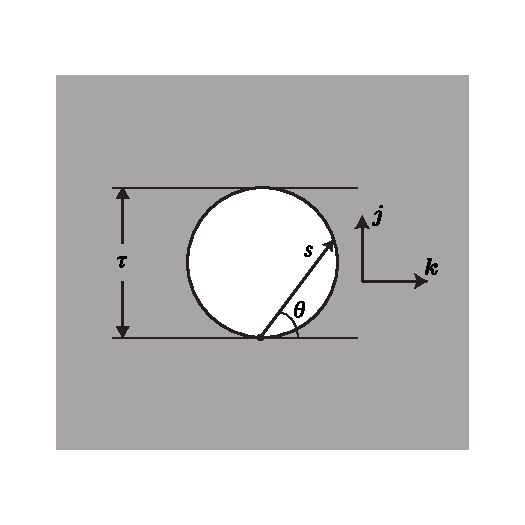
\includegraphics{chord-rz}
%  \caption[A cross-section of the chord length problem in cylindrical
%  geometry.]%
%  {A cross-section of the chord length problem in cylindrical
%  geometry. The orthogonal view looks like Fig.~\ref{fig:chordFlatland}.}
%  \label{fig:chordRz}
%\end{figure}

%%%%%%%%%%%%%%%%%%%%%%%%%%%%%%%%%%%%%%%%%%%%%%%%%%%%%%%%%%%%%%%%%%%%%%%%%%%%%%%%
\clearpage
\section{Transport}

To briefly illustrate the difference between flatland and 2-D geometry, we
view an infinite gap between two materials. The flatland problem and the
two-dimensional projection are identical, shown in Fig.~\ref{fig:chordFlatland}.
%
\begin{figure}[htb]
  \centering
  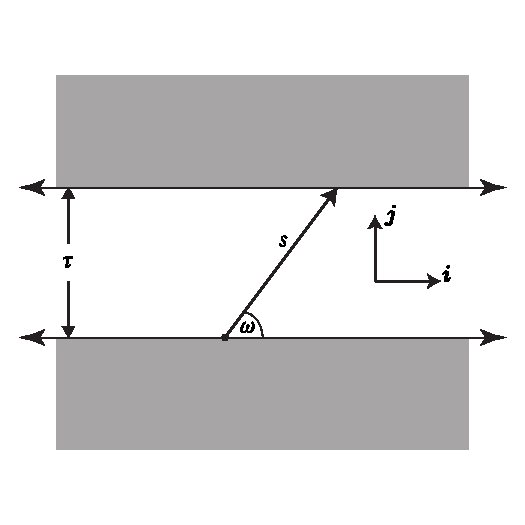
\includegraphics{chord-flatland}
  \caption[The infinite gap as represented on paper.]%
  {The infinite gap as represented on paper. The gap is a distance
  $\tau$ across, $\omega$ is the azimuthal angle, and $s$ is the
  distance across the gap.}
  \label{fig:chordFlatland}
\end{figure}
%
However, in the 2-D case, the figure is merely a slice of a three-dimensional
problem where the two gray rectangles and the gap are infinite in extent
(Fig.~\ref{fig:chordXy}). In the flatland case, the polar angle $\theta$ is
effectively fixed at $\theta=\pi/2$, i.e., $\mu=\cos\theta = 0$.
%
\begin{figure}[htb]
  \centering
  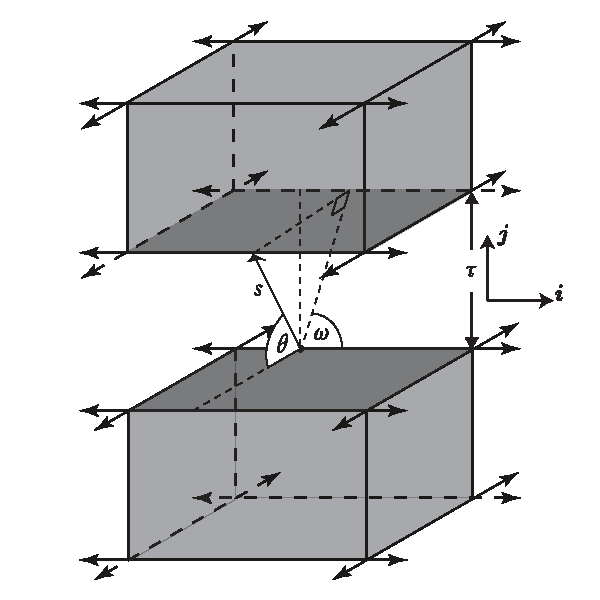
\includegraphics{chord-xyz}
  \caption[A 3-D view of the ``2-D'' infinite gap.]%
  {A 3-D view of the ``2-D'' infinite gap.
  The polar angle cosine is $\mu= \cos \theta$, and the azimuthal angle is
  $\omega$.}
  \label{fig:chordXy}
\end{figure}

Because the time-dependent and nonlinear terms of thermal radiative transfer are
not affected by the choice of geometry, we constrain our discussion in this
section to steady-state transport. Our application of the flatland
transport equation
has only isotropic emission (and ``pseudo-scattering'' if the linearized
transport equation is used), so we limit our study to the case of isotropic
scattering.

To begin, we write the steady-state transport equation with isotropic scattering
in a ``general geometry'' form valid both for flatland and real space (1-D,
2-D, and 3-D):
\begin{subequations} \label{eqs:ssTransport}
\begin{equation}\label{eq:ssTransportVol}
  \vec{\Omega}\vd \grad I(\vec{x}, \vec{\Omega})
  + \sigma(\vec{x}) I(\vec{x}, \vec{\Omega})
  = \frac{c(\vec{x}) \sigma(\vec{x})}{\gamma_0} \phi(\vec{x})
  + \frac{1}{\gamma_0} q(\vec{x}) \,,
  \quad \vec{x} \in V \,,\ \vec{\Omega} \in \Omega\,.
\end{equation}
Here, we use the following definitions:
\begin{align*}
  I(\vec{x},\vec{\Omega}) &= \text{the steady-state angular intensity,} \\
  \vec{\Omega} &= \text{the unit direction vector,} \\
  \Omega &= \text{the domain of the direction vector (the ``unit sphere''),} \\
  \gamma_n &= \text{the $n$th angular moment,} \\
  c(\vec{x}) &= \text{the scattering ratio, and} \\
  \phi(\vec{x}) &= \text{the scalar intensity, i.e.~the zeroth angular moment of $I$.}
\end{align*}
The direction vectors $\vec{\Omega}$ and domains $\Omega$ are presented in
Table~\ref{tab:angularDomain}, and the moments $\gamma_0$ are evaluated in
Table~\ref{tab:angularMoments}. The specified incident radiation
boundary:
\begin{equation} \label{eq:ssBndy}
  I(\vec{x}, \vec{\Omega}) = I^b(\vec{x}, \vec{\Omega})
  \quad \vec{x} \in \partial V \,,\ \vec{\Omega} \vd \vec{n} < 0\,.
\end{equation}
\end{subequations}

\begin{table}[htb]
  \centering
  \begin{tabular}{rccc}
\toprule
   Geometry & $\vec{\Omega}$ & Domain $\Omega$ & $\ud\Omega$
\\ \midrule
   1-D & $\mu$ & $-1 \le \mu \le 1$ & $\ud\mu$
   \\
   2-D & $\sqrt{1-\mu^2} \cos \omega \vec{i}
   + \sqrt{1-\mu^2} \sin \omega \vec{j}$
   & $-1 \le \mu \le 1$, $0 \le \omega < 2\pi$ & $\ud\mu \ud \omega$
   \\
   Flatland & $\cos \omega \vec{i} + \sin \omega \vec{j}$
   & $0 \le \omega < 2\pi$ & $\ud \omega$
   \\
   3-D & $\mu \vec{i}
   + \sqrt{1-\mu^2} \cos \omega \vec{j}
   + \sqrt{1-\mu^2} \sin \omega \vec{k}$
   & $-1 \le \mu \le 1$, $0 \le \omega < 2\pi$ & $\ud\mu \ud \omega$
\\ \bottomrule
  \end{tabular}
  \caption{Angular variables in the various geometries.}
  \label{tab:angularDomain}
\end{table}

\begin{table}[htb]
  \centering
  \begin{tabular}{rccc}
\toprule
   Geometry
   & $\gamma_0 \equiv \int_\Omega \ud\Omega$
   & $\gamma_1 \equiv \int_\Omega \abs{\vec{\Omega}\vd\vec{i}} \ud\Omega$
   & $\gamma_2 \equiv \int_\Omega (\vec{\Omega}\vd\vec{i})^2 \ud\Omega$
\\ \midrule
   1-D & 2 & 1 & $\frac{2}{3}$
   \\
   2-D & $4\pi$ & $2\pi$ & $\frac{4\pi}{3}$
   \\
   Flatland & $2\pi$ & $4$ & $\pi$
   \\
   3-D & $4\pi$ & $2\pi$ & $\frac{4\pi}{3}$
\\ \bottomrule
  \end{tabular}
  \caption{Angular moments in each geometry.}
  \label{tab:angularMoments}
\end{table}

The ``unit sphere''---%
the domain of the unit direction $\vec{\Omega}$---%
differs among the geometries. In 3-D, the direction variable is a unit vector,
$\norm{\vec{\Omega}}=1$, so valid angles
lie on the surface of a sphere of unit radius. In 2-D, those angles are
projected onto a slice through the sphere's middle, so that
$\norm{\vec{\Omega}} \le 1$: valid angles are on a unit disc. Angles on the edge
of the disc---the unit circle---represent particles traveling along the slice,
and angles inside the unit circle are the projection of 3-D angles traveling with a
non-zero polar angle cosine. Flatland geometry allows only angles on the unit
circle, $\norm{\vec{\Omega}}=1$.

%%%%%%%%%%%%%%%%%%%%%%%%%%%%%%%%%%%%%%%%
\subsection{Monte Carlo sampling}

In numerically testing the anisotropic diffusion approximation, we use Monte Carlo
methods to generate the reference solutions.
The Monte Carlo method approximates the transport equation by tracking the
random histories of statistically large numbers of particles as they traverse a
problem. The behavior during their lifetime depends on probability distribution
functions (PDFs) that describe how they are born, how far they travel without a
collision, how they behave when they collide, and so on \cite{Lew1984,Bro2004a}.

In this section, we form and discuss the probability distributions particular to
flatland geometry. We briefly derive those PDFs,
integrate them to get cumulative distribution functions
(CDFs), and use the direct inversion method to show how a uniformly sampled
pseudo-random number $\xi \in [0,1)$ may be used to determine particle behavior
in flatland. Because the geometry tracking routines of steady state Monte Carlo
and Fleck and Cummings' IMC are identical, the results in this section are
applicable any flatland Monte Carlo implementation.

\subsubsection{Isotropic volume source}
A particle emitted from an isotropic internal source, whether an extraneous
radiation source or an indirect isotropic scattering event, has an equal
probability of entering any angle. In any geometry, the normalized PDF that
represents this process is
\begin{equation*}
  f(\vec{\Omega}) \ud \Omega = \alpha \ud \Omega \,,
  \quad \vec{\Omega} \in \Omega \,,
\end{equation*}
where $\Omega$ is the angular domain of the
geometry (see Table~\ref{tab:angularDomain}), and $\alpha$ is a normalization
constant.
Requiring the PDF to integrate to unity over its domain gives the
following value for $\alpha$ in any geometry:
\begin{align*}
  1 = \int_{\Omega} f(\vec{\Omega}) \ud\Omega
  = \alpha \int_{\Omega} \ud\Omega = \alpha \gamma_0
  \lra
  \alpha = \frac{1}{\gamma_0}\,.
\end{align*}
Thus the angular distribution of an isotropic volume source is
\begin{equation}\label{eq:volumeSourcePdf}
  f(\vec{\Omega}) \ud \Omega = \frac{\ud\Omega}{\gamma_0} \,,
  \quad \vec{\Omega} \in \Omega\,.
\end{equation}

In 2-D, using the identities from Tables~\ref{tab:angularDomain}
and~\ref{tab:angularMoments}, Eq.~\eqref{eq:volumeSourcePdf} evaluates to the
familiar
\begin{equation*}
  f(\mu,\omega) \ud\mu\ud\omega = \frac{\ud\mu\ud\omega}{4\pi} 
  = \frac{\ud\mu}{2}\frac{\ud\omega}{2\pi}
  \,,
  \quad -1\le \mu \le 1,\ 0 \le \omega < 2\pi\,,
\end{equation*}
which, integrated, yields the separable CDF
\begin{equation*}
  F(\mu,\omega) = F_1(\mu) F_2(\omega)
  = \frac{1 + \mu}{2}\frac{\omega}{2\pi}\,,
  \quad -1\le \mu \le 1,\ 0 \le \omega < 2\pi\,.
\end{equation*}
Setting two uniformly sampled random numbers $\xi_1 = F_1(\mu)$ and
$\xi_2 = F_2(\omega)$, solving for $\mu$ and $\omega$, and
introducing them back into the 2-D representation of $\vec{\Omega}$, we obtain the
new direction for an isotropically emitted particle in 2-D:
\begin{align*}
  \vec{\Omega} &= \sqrt{1-\mu^2} \cos \omega \vec{i}
  + \sqrt{1-\mu^2} \sin \omega \vec{j}
\\
  &= \sqrt{1-(2\xi_1-1)^2} \cos(2\pi\xi_2) \vec{i}
  + \sqrt{1-(2\xi_1-1)^2} \sin(2\pi\xi_2) \vec{j}\,.
\end{align*}

In flatland, Eq.~\eqref{eq:volumeSourcePdf} becomes the simpler
\begin{equation*}
  f(\omega) \ud\omega = \frac{\ud\omega}{2\pi} \,,
  \quad 0 \le \omega < 2\pi\,,
\end{equation*}
yielding the CDF
\begin{equation}\label{eq:volumeSourceFlatland}
  F(\omega) = \frac{\omega}{2\pi}\,,
  \quad 0 \le \omega < 2\pi\,,
\end{equation}
Setting $\xi_1 = F(\omega)$ and solving for $\omega = F\inv(\xi_1)$ gives the
following simple relation between an isotropically sampled angle $\omega$ and a
uniformly sampled random number $\xi_1$:
\begin{equation*}
  \omega = 2\pi \xi_1\,.
\end{equation*}
The flatland particle's new angle is therefore
\begin{equation*}
  \vec{\Omega} = \cos \omega \vec{i} + \sin \omega \vec{j}
  = \cos(2\pi\xi_1) \vec{i} + \sin(2\pi\xi_1) \vec{j}\,.
\end{equation*}

With only one independent variable that needs sampling, and the omission of
the transcendental operation $\sqrt{1-\mu^2}$, the computational cost of a
scattering event is less in flatland than in 2-D, leading to
faster simulation times.

\subsubsection{Isotropic surface source}\label{sec:isoSurface}
Particles emitted from an isotropic surface source have a cosine distribution
\cite{Gre2002}, where the partial first moment in each differential angle is
constant. The PDF for a surface source is
\begin{equation*}
  f(\vec{\Omega}) \ud \Omega = \alpha \abs{\vec{\Omega}\vd \vec{n}} \ud \Omega \,,
\quad \vec{\Omega}\vd \vec{n} < 0 \,,
\end{equation*}
where $\alpha$ is a normalization constant. We obtain $\alpha$ by integrating over
the angular domain and substituting the angular moments from Table~\ref{tab:angularMoments}:
\begin{align*}
  1 &= \int_{\vec{\Omega}\vd \vec{n} < 0} \left[ \alpha \abs{\vec{\Omega}\vd
  \vec{n}} \right] \ud\Omega
  \\
  1 &=\frac{\alpha}{2} \int_{\Omega} \abs{\vec{\Omega}\vd \vec{n}} \ud\Omega
  \\
  \alpha &= \frac{2}{\gamma_1}\,.
\end{align*}
Thus, the normalized PDF for an isotropic surface source is
\begin{equation}\label{eq:surfaceSourcePdf}
  f(\vec{\Omega}) \ud \Omega = \frac{2}{\gamma_1} \abs{\vec{\Omega}\vd \vec{n}} \ud \Omega \,,
\quad \vec{\Omega}\vd \vec{n} < 0 \,.
\end{equation}

In 3-D, choosing $\vec{n}=\vec{i}$, the isotropic surface PDF is
\begin{equation*}
  f(\mu,\omega) \ud\mu \ud\omega
  = \frac{1}{\pi} \mu \ud\mu \ud\omega
  = (2 \mu \ud\mu) \frac{\ud\omega}{2\pi}\,,
\end{equation*}
which gives the separable CDF
\begin{equation*}
  F(\mu,\omega) = \mu^2 \frac{\omega}{2\pi}\,.
\end{equation*}
The sampled directions are thus $\mu=\sqrt{\xi_1}$ and $\omega=2\pi \xi_2$.

In flatland, the surface source distribution is different. Let us choose
$\vec{n} = -\vec{j}$ so that emitted particles have azimuthal angles in the range
$\omega \in [0, \pi)$.
Applying the flatland identities in Tables~\ref{tab:angularDomain}
and~\ref{tab:angularMoments} to Eq.~\eqref{eq:surfaceSourcePdf}, we obtain
the following surface source PDF for flatland:
\begin{equation*}
  f(\omega) \ud\omega = \frac{2}{4} \, \abs{ -\sin \omega}\ud\omega
  = \frac{1}{2} \sin \omega\ud\omega \,,\quad 0 \le \omega < \pi\,.
\end{equation*}
The corresponding CDF is
\begin{equation}\label{eq:surfaceSourceFlatland}
  F(\omega) = \frac{1}{2} \left( 1-\cos\omega \right)
  \,,\quad 0 \le \omega < \pi\,.
\end{equation}
Solving for $\omega = F\inv(\xi_1)$ gives the sampled azimuthal angle for a surface source
in flatland:
\begin{equation*}
  \omega = \cos\inv(1 - 2\xi_1)\,.
\end{equation*}
Finally, we insert this sampled angle into the flatland
direction vector $\vec{\Omega}$ and use the identity
$\cos^2 \omega + \sin^2 \omega = 1$ to reduce the number of transcendental
functions. Thus the sampled direction of a particle from an isotropic surface
source is:
\begin{align*}
  \vec{\Omega} &= \cos \omega \vec{i} + \sin \omega \vec{j} \\
  &=  \cos[ \cos\inv(1 - 2\xi_1) ] \vec{i} + \sin[ \cos\inv(1 - 2\xi_1) ] \vec{j} \\
  &= (1 - 2\xi_1) \vec{i} + \sqrt{1 - (1 - 2\xi_1)^2} \vec{j}\,.
\end{align*}

%%%%%%%%%%%%%%%%%%%%%%%%%%%%%%%%%%%%%%%%
\subsection{Discrete ordinates quadrature}

A standard practice in two-dimensional discrete ordinates (\SN) solvers is to
create a quadrature set with polar angles that encompass only the top half of a
unit sphere, $\mu>0$, and to modify the ordinate weights so that they sum to
$4\pi$
\cite{Zik1997}. An ideal quadrature set will also correctly integrate the
angular moments of Table~\ref{tab:angularMoments}:
\begin{equation*}
  \gamma_n \approx \sum_{m=1}^{M} \abs{ \vec{\Omega}_m \vd \vec{i}}^n w_m\,.
\end{equation*}

The most straightforward way of implementing a \emph{flatland} \SN\
code with only isotropic scattering is to use an existing 2-D \SN\ code with a
special quadrature set
consisting of ordinates that have a single
polar angle $\mu=0$. To retain compatibility with the isotropic scattering
kernel, the quadrature weights are normalized so that they sum to $4\pi$
instead of $2\pi$.

As an example, let us consider the calculation of the anisotropic diffusion tensor
in a homogeneous medium.  The purely absorbing flatland transport problem has the
solution $f(\vec{\Omega}) = \frac{1}{2\pi\sigma}$, which yields the diffusion
coefficient
\begin{equation*}
  \Dtens = \int_{0}^{2\pi} \vec{\Omega}\vec{\Omega} f(\vec{\Omega}) \ud \omega
  = \frac{1}{2\sigma} \Identitytens \,.
\end{equation*}
In an \SN\ calculation implemented with modified quadrature weights, the
transport solution for each angle $m$ will yield $f_m = \frac{1}{4\pi\sigma}$,
but the quadrature integration will yield
\begin{equation*}
  \Dtens = \sum_{m=1}^{M} \vec{\Omega}_m \vec{\Omega}_m f_m  w_m 
  = \frac{1}{2\sigma} \Identitytens \,.
\end{equation*}
This implementation therefore will calculate the correct angular moments of
the transport solution, but the apparent value of each $f_m$ is one half 
the correct value. Thus, for example, visualizing the \SN\
solution by plotting $f_m$ as a function of $\omega_m$ requires multiplying by a
factor of two.

%This scaling has two notable side effects. First, because the weights are twice
%what they should be, the \SN\ angular moments approach twice the flatland
%moments $\gamma_n$:
%\begin{equation*}
%  2 \gamma_n \approx \sum_{m=1}^{N} w_m \abs{ \vec{\Omega}_m \vd \vec{i}}^n \,.
%\end{equation*}

% Here is an
%example that uses the \verb|matplotlib| Python module's polar plot to view
%the flatland angular intensity:
%\begin{verbatim}
%    polar( [ angle.getPhi() for angle in quadrature_set ],
%           [ 2 * value for value in psi ] )
%\end{verbatim}

%%%%%%%%%%%%%%%%%%%%%%%%%%%%%%%%%%%%%%%%%%%%%%%%%%%%%%%%%%%%%%%%%%%%%%%%%%%%%%%%
\section{Diffusion}

An accurate flatland diffusion formulation
is needed for benchmarking the anisotropic diffusion
approximation against diffusion solutions.
In the following section we derive ``Marshak'' and ``variational'' boundary
conditions for the flatland diffusion equation. (A summary of this original
work is published in \cite{Joh2011a}.)
%There is no loss of generality in
%ignoring the time dependence because of the quasi-static approximation made in
%the derivation of the diffusion coefficient (see \S\ref{sec:bgDiffusion}).

The difference between diffusion in flatland and 2-D results from the
angular moments in the two geometries, which
are defined (and evaluated in Table~\ref{tab:angularMoments}) as:
\begin{equation*}
  \gamma_n \equiv \int_\Omega \abs{\vec{\Omega} \vd \vec{i}}^n \ud \Omega\,.
\end{equation*}
These give rise not only to a different diffusion coefficient in the interior
but also different boundary conditions.

%%%%%%%%%%%%%%%%%%%%%%%%%%%%%%%%%%%%%%%%
\subsection{Interior diffusion approximation}

The diffusion approximation begins by assuming that $I$ is linear in angle:
\begin{equation*}
  I(\vec{x}, \vec{\Omega}) \approx f(\vec{x}) + \vec{\Omega} \vd
  \vec{g}(\vec{x})\,.
\end{equation*}
The zeroth angular moment of $I$ determines $f$:
\begin{equation*}
  \phi = \int_\Omega I \ud \Omega
= \int_\Omega \left( f + \vec{\Omega}\vd \vec{g} \right) \ud\Omega
= \int_\Omega\ud\Omega f + 0
= \gamma_0 f \,,
\end{equation*}
and the first moment of $I$ determines $g$:
\begin{equation*}
  \vec{F} = \int_\Omega \vec{\Omega} I \ud \Omega
= f \int_\Omega \vec{\Omega} \ud\Omega
  + \vec{g} \vd \int_\Omega \vec{\Omega}\vec{\Omega} \ud\Omega
= \gamma_2 \vec{g} \,.
\end{equation*}
This is the \Pone\ approximation to the radiation intensity:
\begin{equation}\label{eq:ssPone}
  I(\vec{x}, \vec{\Omega})
  \approx \frac{1}{\gamma_0} \phi(\vec{x})
  + \frac{1}{\gamma_2} \vec{\Omega} \vd \vec{F}(\vec{x})\,.
\end{equation}

The diffusion approximation is a closure for the first angular moment of
the transport equation. Operating on Eq.~\eqref{eq:ssTransportVol} by
$\int_\Omega \vec{\Omega} (\cdot) \ud \Omega$ and substituting
the approximation in Eq.~\eqref{eq:ssPone} reduces the first angular moment of
the transport equation to the following:
\begin{align*}
  \grad \vd \int_\Omega \vec{\Omega} \vec{\Omega} I
  \ud\Omega
  + \sigma \int_\Omega \vec{\Omega} I \ud\Omega
  &=
  \frac{c\sigma}{\gamma_0} \phi \int_\Omega \vec{\Omega} \ud\Omega
  + \frac{1}{\gamma_0} q \int_\Omega \vec{\Omega} \ud\Omega
  \\
  \grad \vd \int_\Omega \vec{\Omega} \vec{\Omega} \left(
  \frac{1}{\gamma_0}\phi + \frac{1}{\gamma_2} \vec{\Omega} \vd \vec{F}
  \right)
  \ud\Omega
  + \sigma \vec{F}
  &= 0
  \\
  \frac{1}{\gamma_0} \grad \vd \int_\Omega \vec{\Omega} \vec{\Omega}
  \ud\Omega\, \phi 
  + \sigma \vec{F} &= 0
  \\
  \frac{\gamma_2}{\gamma_0} \grad \phi + \sigma \vec{F} &= 0 \,.
\end{align*}
Solving for $\vec{F}$ gives Fick's law, expressed in the general form:
\begin{equation} \label{eq:fickGeneral}
  \vec{F}(\vec{x})
  = - \frac{\gamma_2}{\gamma_0} \frac{1}{\sigma(\vec{x})} \grad \phi(\vec{x})
  \equiv -D(\vec{x}) \grad \phi(\vec{x})\,.
\end{equation}
In 2-D and 3-D, $\gamma_2/\gamma_0 = (4\pi / 3) / (4\pi) = 1/3$; in
flatland, $\gamma_2/\gamma_0 = \pi / (2\pi) = 1/2$. Thus, $D=\frac{1}{3\sigma}$ in
2-D but $D=\frac{1}{2\sigma}$ in flatland.

Substituting Fick's law into the linear-in-angle approximation,
Eq.~\eqref{eq:ssPone}, we obtain the diffusion approximation to the angular
intensity:
\begin{align} \nonumber
  I(\vec{x}, \vec{\Omega})
  &\approx \frac{1}{\gamma_0} \phi(\vec{x})
  + \frac{1}{\gamma_2} \vec{\Omega} \vd \left[ - \frac{\gamma_2}{\gamma_0}
  \frac{1}{\sigma(\vec{x})} \grad \phi(\vec{x}) \right]
  \\ \label{eq:diffusionIntensity}
  I(\vec{x}, \vec{\Omega})
  &= \frac{1}{\gamma_0} \left[ \phi(\vec{x})
  - \frac{1}{\sigma(\vec{x})}
  \vec{\Omega} \vd \grad \phi(\vec{x}) \right] \,.
\end{align}
In physical geometry this is the standard diffusion approximation
\begin{equation*}
 I(\vec{x}, \vec{\Omega})
= \frac{1}{4\pi} \left[ \phi(\vec{x}) - \frac{1}{\sigma(\vec{x})} \vec{\Omega}
\vd \grad \phi(\vec{x}) \right] \,,
\end{equation*}
and in flatland, the diffusion approximation is
\begin{equation}\label{eq:flatlandDiffusion}
 I(\vec{x}, \vec{\Omega})
= \frac{1}{2\pi} \left[ \phi(\vec{x}) - \frac{1}{\sigma(\vec{x})} \vec{\Omega}
\vd \grad \phi(\vec{x}) \right]\,.
\end{equation}

%%%%%%%%%%%%%%%%%%%%%%%%%%%%%%%%%%%%%%%%
\subsection{Marshak boundary condition}
The Marshak boundary condition \cite{Mar1947} preserves the incident radiation
flux (the partial first moment for incoming directions) on the boundary. It is
derived by substituting the approximate diffusion
intensity from Eq.~\eqref{eq:diffusionIntensity} into the boundary condition,
Eq.~\eqref{eq:ssBndy}, multiplying by $\abs{\vec{\Omega}\vd \vec{n}}$, and integrating over
incident directions:
\begin{align*}
\int_{\vec{\Omega}\vd \vec{n} < 0 } \abs{\vec{\Omega}\vd \vec{n}}
I^b \ud\Omega
 &= 
\int_{\vec{\Omega}\vd \vec{n} < 0 } \abs{\vec{\Omega}\vd \vec{n}} 
 \frac{1}{\gamma_0} \left[ \phi - \frac{1}{\sigma}
  \vec{\Omega} \vd \grad \phi \right]
  \ud\Omega
\\
F^{-}
&= 
\frac{1}{\gamma_0} \phi \left( \int_{\vec{\Omega}\vd \vec{n} < 0 }
\abs{\vec{\Omega}\vd \vec{n}} \ud\Omega \right) 
  - \frac{1}{\gamma_0}\frac{1}{\sigma}
  \left( \int_{\vec{\Omega}\vd \vec{n} < 0 } [-\vec{\Omega}\vd \vec{n}]
  \vec{\Omega} \ud\Omega  \right) \vd \grad \phi
\\
F^{-}
&=
\frac{1}{\gamma_0} \phi \left( \frac{\gamma_1}{2} \right) 
  + \frac{1}{\gamma_0}\frac{1}{\sigma} \left( \vec{n} \vd
  \frac{\gamma_2}{2} \Identitytens \right)
  \vd \grad \phi
\\
F^{-}
&=
\frac{\gamma_1}{2\gamma_0} \phi
+ \frac{\gamma_2}{2\gamma_0}\frac{1}{\sigma} \vec{n} \vd \grad \phi\,.
\end{align*}
This is the Marshak diffusion boundary condition:
\begin{equation} \label{eq:marshak}
\frac{2\gamma_0}{\gamma_1} F^{-}
=
\phi + \frac{\gamma_2}{\gamma_1}\frac{1}{\sigma} \vec{n} \vd \grad \phi\,.
\end{equation}

The value
\begin{equation*}
  \frac{\gamma_2}{\gamma_1}
  =
  \begin{cases}
    \frac{2}{3} \approx 0.6667 & \text{in 1-D, 2-D, 3-D; and} \\
    \frac{\pi}{4} \approx 0.7854 & \text{in flatland,}
  \end{cases}
\end{equation*}
is the Marshak extrapolation distance.
The underlying physical reason for the longer extrapolation distance in flatland
is that in 2-D, a greater fraction of particles travel at a steep angle to the
$x,y$-plane, yielding a steeper slope for $\phi$ on the boundary.

We can also rewrite the Marshak boundary condition in terms of the diffusion
coefficient by substituting $D$ from Eq.~\eqref{eq:fickGeneral}:
\begin{equation*}
\frac{2\gamma_0}{\gamma_1} F^{-}
= \phi + \frac{\gamma_0}{\gamma_1} D \vec{n} \vd \grad \phi\,.
\end{equation*}
In 1-D, 2-D, and 3-D geometries, this is the standard Marshak boundary condition
\begin{equation*}
4 F^{-}
= \phi + 2 D \vec{n} \vd \grad \phi\,.
\end{equation*}
In flatland, it is the following:
\begin{equation}\label{eq:flatMarshak}
\pi F^{-}
= \phi + \frac{\pi}{2} D \vec{n} \vd \grad \phi\,.
\end{equation}

%%%%%%%%%%%%%%%%%%%%%%%%%%%%%%%%%%%%%%%%
\subsection{Variational boundary condition} \label{sec:varBndy}
It is known that the Marshak boundary condition is heuristic and that
a more accurate boundary condition for diffusion can be derived from an
asymptotic matched boundary layer analysis. However, a simpler
method of deriving a more accurate (than Marshak) boundary condition is to use
a variational analysis \cite{Mal1991}.
A shorter but equivalent analysis, adapted to flatland geometry, follows.

%A lengthy asymptotic boundary layer
%matching analysis \cite{Hab1975} shows that the correct weighting of the
%boundary condition is not $\abs{\vec{\Omega}\vd\vec{n}}$ but rather
%$W(\abs{\vec{\Omega}\vd\vec{n}})$, where $W$ is related to Chandrasekhar's
%$H$-function \cite{Cha1960}:
%\begin{equation*}
%  W(\mu) = \frac{\sqrt{3}}{2} \mu H(\mu) \,,
%\end{equation*}
%which gives an extrapolation distance of
%\begin{align*}
%  z_0 = \frac{\int_{0}^{1} \mu W(\mu) \ud \mu}{\int_{0}^{1} W(\mu) \ud
%  \mu} \approx 0.7104\,.
%\end{align*}
%
%A variational analysis \cite{Mal1991} has been used to
%derive a very accurate approximation to $W$:
%\begin{equation*}
%W(\mu) \approx \mu + \tfrac{3}{2} \mu^2 \,,
%\end{equation*}
%which gives the approximate extrapolation distance of
%\begin{equation*}
%  z_0 = \frac{\int_{0}^{1} \mu (\mu + \tfrac{3}{2} \mu^2 ) \ud
%  \mu}{\int_{0}^{1} (\mu + \tfrac{3}{2} \mu^2 ) \ud \mu} 
%  = \frac{17}{24} \approx 0.7083 \,.
%\end{equation*}

We consider a homogeneous, source-free ($q=0$), purely scattering ($c=1$)
transport problem in a
semi-infinite flatland plane.\footnote{%
The justification for setting $c=1$ and $q=0$ relates to the asymptotic
scaling used to derive diffusion from the transport equation:
both $q$ and $1-c$ are $O(\epsilon^2)$ quantities \cite{Mal1991}.}
The transport equation~\eqref{eq:ssTransportVol} becomes
\begin{subequations} \label{eqs:flatTransport}
\begin{equation}\label{eq:flatTransportVol}
  \cos \omega \pder{I}{x} + \sin \omega \pder{I}{y} + \sigma I
  = \frac{\sigma}{2\pi} \int_{0}^{2\pi} I \ud \omega'\,,\quad
 -\infty < x < \infty,\ 0 \le y < \infty,\ 0 \le \omega < 2\pi\,.
\end{equation}
It has a uniform incident boundary condition,
\begin{equation}\label{eq:flatTransportBndy}
  I(x, 0, \omega) = I^b(\omega) \,,\quad -\infty < x < \infty,\ 
  0 \le \omega < \pi \,.
\end{equation}
\end{subequations}
%The justification for using a purely scattering problem is related to the
%asymptotic analysis that shows the transport solution to satisfy a diffusion
%equation in the ``diffusive'' limit. In this limit, absorption is scaled as
%$O(\epsilon^2)$; the full variational analysis \cite{Mal1991} yields a
%variational estimate of the transport solution also accurate to $O(\epsilon^2)$.

Because neither the boundary condition nor $\sigma$ varies
in $x$, $\tpder{I}{x}=0$, and Eq.~\eqref{eq:flatTransportVol} reduces to the
one-dimensional flatland transport equation 
\begin{equation*}
  \sin \omega \pder{}{y}I(y,\omega) + \sigma I(y,\omega)
  = \frac{\sigma}{2\pi} \int_{0}^{2\pi} I(y,\omega') \ud \omega'\,.
\end{equation*}
which is \emph{not} the 1-D planar geometry transport equation.

We define the $y$ components of the angular moments of $I$ as
\begin{equation} \label{eq:flatPhi}
  \phi_m(y) = \int_{0}^{2\pi} (\vec{\Omega}\vd\vec{j})^m I(y,\omega) \ud\omega
  = \int_{0}^{2\pi} (\sin\omega)^m I(y,\omega) \ud\omega \,.
\end{equation}
As $y\to\infty$, the intensity $I$ will approach a constant $\varphi/2\pi$,
which gives $\phi_0(\infty)=\phi(\infty)\equiv\varphi$.
Concordantly, $\phi_1(\infty)=0$.

Operating on the transport equation by $\int_{0}^{2\pi} (\sin\omega)^m (\cdot)
\ud\omega$ gives the $m$th angular moment in the $y$ direction:
\begin{align} \nonumber
  \pder{}{y} \int_{0}^{2\pi} (\sin\omega)^{m+1} I \ud\omega
  + \sigma \int_{0}^{2\pi} (\sin\omega)^{m} I \ud\omega
  &= \frac{\sigma}{2\pi} \int_{0}^{2\pi} I \ud \omega'
  \int_{0}^{2\pi} (\sin\omega)^{m} \ud\omega
  \\ \label{eq:flatMoments}
  \pder{\phi_{m+1}}{y}
  + \sigma \phi_{m}
  &= \frac{\sigma}{2\pi} \phi_{0}
  \int_{0}^{2\pi} (\sin\omega)^{m} \ud\omega\,.
\end{align}
For $m=0$, the conservation equation, Eq.~\eqref{eq:flatMoments} evaluates to
\begin{equation*}
  \pder{\phi_{1}}{y}
  + \sigma \phi_{0}
  = \frac{\sigma}{2\pi} \phi_{0} (2\pi)
  \lra
  \pder{\phi_{1}}{y} = 0\,.
\end{equation*}
In other words, the radiation flux is a constant, and because $\phi_1(\infty)=0$,
that constant is zero. Physically, a constant $\phi_1$ means that at every
point, the rate of energy being transferred away from the boundary is balanced
by energy moving toward the boundary. This logically follows from the lack of
absorption in the problem: at steady-state, the only means of energy loss is
through exiting the boundary.

Evaluating Eq.~\eqref{eq:flatMoments} for $m=1$ and using the result that
$\phi_{1}=0$, we obtain
\begin{equation*}
  \pder{\phi_{2}}{y}
  + \sigma \phi_{1}
  = \frac{\sigma}{2\pi} \phi_{0} (0)
  \lra
  \pder{\phi_{2}}{y} = 0\,.
\end{equation*}
Thus $\phi_{2}$ is also a constant. At large distances from the boundary,
$y\to\infty$, the radiation assumes an isotropic distribution,
$I\to\varphi/2\pi$. From these two facts we relate the second angular moment
throughout the problem to the equilibrium scalar intensity $\varphi$:
\begin{equation*}
  \phi_{2} = \int_{0}^{2\pi} (\sin\omega)^2 \frac{\varphi}{2\pi} \ud\omega
  = \frac{1}{2} \varphi\,.
\end{equation*}
% in 1-D, this would be $\int_{-1}^{1}\mu^2\frac{\varphi}{2} \ud \mu =
% \frac{1}{3} \varphi$.

Since $\phi_1=0$, we can add $\alpha \phi_1$ to the previous equation for any
$\alpha$:
\begin{align*}
 \alpha\phi_1 + \phi_{2} &= \frac{\varphi}{2} \\
 \int_{0}^{2\pi} (\alpha \sin\omega + \sin^2\omega)
 I(y,\omega) \ud\omega
 &= \frac{\varphi}{2}\,.
\end{align*}
At the boundary $y=0$, $I=I^b$ for incident angles $0 \le \omega < \pi$.
The variational analysis in \cite{Mal1991} reveals that certain trial functions
allow an exiting angular distribution that is isotropic to second order accuracy,
so we make the ``variational'' approximation that $I(0,\omega)=I^\text{out}$.
The previous equation then yields
\begin{equation*}
 \int_{0}^{\pi} (\alpha \sin\omega + \sin^2\omega)
 I^b(\omega) \ud\omega
 + \int_{\pi}^{2\pi} (\alpha \sin\omega + \sin^2\omega)\ud\omega I^\text{out}
 = \frac{\varphi}{2}\,.
\end{equation*}
The value $\alpha=\pi/4$ eliminates the integral over outgoing directions and
gives the following relation between moments of the incident angular flux and the
magnitude of the angular flux as $y\to\infty$:
\begin{equation}\label{eq:varBoundary}
 \varphi = 2\int_{0}^{\pi} \left( \frac{\pi}{4} \sin\omega + \sin^2\omega \right)
 I^b(\omega) \ud\omega
 \,.
\end{equation}

We wish our boundary condition to preserve the value of
$\varphi$ when the diffusion method is used, so we substitute the diffusion
approximation, Eq.~\eqref{eq:flatlandDiffusion}:
\begin{align*}
 \varphi &= 2\int_{0}^{\pi} \left( \frac{\pi}{4} \sin\omega + \sin^2\omega \right)
 I^b(\omega) \ud\omega
 \\
 &= 
  2\int_{0}^{\pi} \left( \frac{\pi}{4} \sin\omega + \sin^2\omega \right)
 \left( \frac{1}{2\pi} \phi -
  \frac{1}{\sigma} \sin\omega \pder{\phi}{y}\right)\ud\omega
\\
 &= 
\frac{1}{2\pi} \int_{0}^{\pi} \left( \frac{\pi}{2} \sin\omega + 2 \sin^2\omega
\right)\ud\omega
 \,\phi -
 \frac{1}{2\pi} \int_{0}^{\pi} \left( \frac{\pi}{2} \sin^2\omega + 2 \sin^3\omega \right)\ud\omega
  \,\frac{1}{\sigma} \pder{\phi}{y}
  \\
 &= 
 \frac{1}{2\pi} \left( \frac{\pi}{2} [2] + 2 \frac{\pi}{2}
\right) \phi
-
\frac{1}{2\pi} \left( \frac{\pi}{2} \left[ \frac{\pi}{2} \right] + 2 \left[
\frac{4}{3} \right] \right) \frac{1}{\sigma} \pder{\phi}{y}
\\
 &= 
  \phi
- \left( \frac{\pi}{8} + \frac{4}{3\pi} \right) \frac{1}{\sigma} \pder{\phi}{y}
\,.
\end{align*}
In this problem, the boundary surface outer normal is $\vec{n}=-\vec{j}$. 
Replacing $\sin \omega$ with $-\vec{\Omega}\vd\vec{n}$, we obtain the following
flatland variational boundary condition:
\begin{equation} \label{eq:flatVarBc}
\int_{\vec{\Omega}\vd\vec{n} < 0} \left[ \frac{\pi}{2}
\abs{\vec{\Omega}\vd\vec{n}} + 2 (\vec{\Omega}\vd\vec{n})^2 \right]
I^b(\vec{x}, \vec{\Omega}) \ud\Omega
= 
  \phi_0(\vec{x})
  - \left( \frac{\pi}{8} + \frac{4}{3\pi} \right) \frac{1}{\sigma}
  \vec{n}\vd\grad \phi_0(\vec{x})\,.
\end{equation}
Compared to the flatland Marshak boundary condition,
Eq.~\eqref{eq:flatMarshak}, the variational boundary condition not only yields a
different extrapolation distance $\frac{\pi}{8} + \frac{4}{3\pi} \approx
0.8171$ but also uses a different moment of the incident boundary flux.

%Essentially, we have shown that the flatland equivalent of the $W$ function,
%which we shall call $V$, can be approximated by
%\begin{equation}\label{eq:flatlandVariational}
%  V(\omega)
%  \approx \frac{1}{4}\sin\omega + \frac{1}{\pi} \sin^2\omega \,,\quad
%  0 \le \omega < \pi \,,
%\end{equation}
%which satisfies
%\begin{equation*}
%  \int_{0}^{\pi} V(\omega) \ud\omega= 1
%\end{equation*}
%and gives the extrapolation distance
%\begin{equation*}
%  z = \frac{\int_{0}^{\pi} \sin \omega V(\omega) \ud\omega}{\int_{0}^{\pi}
%  V(\omega) \ud\omega} =  \frac{\pi}{8} + \frac{4}{3\pi} \,.
%\end{equation*}

%%%%%%%%%%%%%%%%%%%%%%%%%%%%%%%%%%%%%%%%%%%%%%%%%%%%%%%%%%%%%%%%%%%%%%%%%%%%%%%%
\section{Anisotropic diffusion}
The derivation of the anisotropic diffusion method presented in
chapter~\ref{chap:adDerivation} needs little modification to be formulated
in the flatland geometry. The most notable change is in formulating the
low-order boundary conditions.

TODO

%
%We begin with a time-dependent transport equation with isotropic scattering,
%using the angular moments from Table~\ref{tab:angularMoments}:
%\begin{subequations} \label{eqs:flatfullTransport}
%\begin{multline} \label{eq:flatfullTransportVol}
%  \frac{1}{c} \pder{I}{t}(\vec{x}, \vec{\Omega}, t)
%    + \vec{\Omega}\vd \grad I(\vec{x}, \vec{\Omega}, t)
%    + \sigmast(\vec{x}) I (\vec{x}, \vec{\Omega}, t)
%    \\ = \frac{1}{\gamma_0} \sigmast(\vec{x}) ac [T(\vec{x}, t)]^4
%    + \frac{1}{\gamma_0} q_{r}(\vec{x}, t)
%    \equiv \frac{1}{\gamma_0} Q(\vec{x}, t) \,,
%\\
%x \in V,\  0 \le t \le \Delta_t, \ \vec{\Omega} \in \Omega\,.
%\end{multline}
%We take the case of an incident radiation source on the boundary:
%\begin{equation} \label{eq:flatfullTransportBndy}
%  I(\vec{x}, \vec{\Omega}, t) = I^b(\vec{x}, \vec{\Omega}, t) \,,
% \quad \vec{x} \in \partial V, \ \vec{\Omega} \vd \vec{n} < 0,
% \ 0 \le t \le \Delta_t\,.
%\end{equation}
%The intensity has the initial condition
%\begin{equation} \label{eq:flatfullTransportInit}
% I(\vec{x}, \vec{\Omega}, 0) = I^i(\vec{x}, \vec{\Omega}) \,,
% \quad \vec{x} \in V, \ \vec{\Omega} \in \Omega\,,
%\end{equation}
%which is usually the solution from the previous time step.
%\end{subequations}
%For the sake of simplicity, we do not consider reflecting boundaries, as their
%formulation is identical to the previous derivation of the AD approximation.
%
%Operating on Eq.~\eqref{eq:flatfullTransportVol} by $\int_{\Omega} (\cdot) \ud
%\Omega$ gives the radiation energy conservation equation,
%\begin{subequations} \label{eqs:flatloEquations}
%\begin{equation} \label{eq:flatloVol}
%\frac{1}{c} \pder{\phi}{t} (\vec{x}, t)
%  + \grad \vd\vec{F}(\vec{x}, t)
%  + \sigmast(\vec{x}) \phi(\vec{x}, t)
%  = \sigmast(\vec{x}) ac [T(\vec{x}, t)]^4 + q_{r}(\vec{x}, t)
%  = Q(\vec{x}, t)\,,
%\end{equation}
%for $\vec{x} \in V$ and $0 \le t \le \Delta_t$.
%Doing the same to the initial condition, Eq.~\eqref{eq:flatfullTransportInit}, gives 
%\begin{equation} \label{eq:flatloInit}
%\phi(\vec{x}, 0) = \int_{\Omega}  I^i(\vec{x},
%\vec{\Omega}) \ud\Omega = \phi^i(\vec{x})\,, \qquad \vec{x} \in V  \,.
%\end{equation}
%\end{subequations}
%Adding $\vec{\Omega}\vd \grad \phi$ to both sides of Eq.~\eqref{eq:flatloVol},
%multiplying by $\frac{1}{\gamma_0}$, and subtracting from
%Eq.~\eqref{eq:flatfullTransportVol}, the isotropic radiation source cancels, leaving
%\begin{equation} \label{eq:flatcapPsiVol}
%  \frac{1}{c} \pder{}{t}\Psi(\vec{x}, \vec{\Omega}, t)
%    + \vec{\Omega}\vd \grad \Psi(\vec{x}, \vec{\Omega}, t)
%    + \sigmast(\vec{x}) \Psi(\vec{x}, \vec{\Omega}, t)
%  = \frac{1}{\gamma_0} \grad \vd\vec{F}(\vec{x}, t) -
%  \frac{1}{\gamma_0} \vec{\Omega}\vd \grad \phi(\vec{x}, t)\,,
%\end{equation}
%where we have defined
%\begin{equation} \label{eq:flatcapPsi}
%  \Psi(\vec{x}, \vec{\Omega}, t) \equiv I(\vec{x}, \vec{\Omega}, t) -
%  \frac{1}{\gamma_0} \phi(\vec{x}, t)\,.
%\end{equation}
%As before, by construction, the zeroth angular moment of $\Psi$ is zero, and its first
%angular moment is $\vec{F}$.
%
%Subtracting $\phi/\gamma_0$ from Eq.~\eqref{eq:flatfullTransportBndy} gives the
%boundary condition
%\begin{equation} \label{eq:flatcapPsiBndy}
% \Psi(\vec{x}, \vec{\Omega}, t) 
%  =I^b(\vec{x}, \vec{\Omega}, t) - \frac{1}{\gamma_0} \phi(\vec{x}, t)\,,
%\end{equation}
%and subtracting from Eq.~\eqref{eq:flatfullTransportInit} gives the initial
%condition
%\begin{equation} 
%\label{eq:flatcapPsiInit}
% \Psi(\vec{x}, \vec{\Omega}, 0)
% = I^i(\vec{x}, \vec{\Omega}) - \frac1{\gamma_0} \phi^i(\vec{x})
% \equiv \Psi^i(\vec{x}, \vec{\Omega}, t)
% \,.
%\end{equation}
%Equations \eqref{eq:flatcapPsiVol},~\eqref{eq:flatcapPsiBndy},
%and~\eqref{eq:flatcapPsiInit} form the transport
%equation for $\Psi$.
%
%%%%%%%%%%%%%%%%%%%%%%%%%%%%%%%%%%%%%%%%%
%\subsection{Interior and boundary layer transport equations}
%
%We separate $\Psi$ into an interior solution $\tilde\Psi$ and a boundary layer
%solution $\Psi_\mathrm{bl}$:
%\begin{equation} \label{eq:flatboundaryLayerPsi}
%  \Psi(\vec{x}, \vec{\Omega}, t)
%  = \tilde\Psi(\vec{x}, \vec{\Omega}, t)
%  + \Psi_\mathrm{bl}(\vec{x}, \vec{\Omega}, t)\,,
%\end{equation}
%defined so that the boundary solution tends rapidly to zero away from the
%problem's exterior surface.
%
%\begin{subequations} \label{eqs:flattCapPsi}
%  The interior transport equation accounts for the right hand side of the equation:
%\begin{multline} \label{eq:flattCapPsiVol}
%  \frac{1}{c} \pder{}{t}\tilde\Psi(\vec{x}, \vec{\Omega}, t)
%    + \vec{\Omega}\vd \grad \tilde\Psi(\vec{x}, \vec{\Omega}, t)
%    + \sigmast(\vec{x}) \tilde\Psi(\vec{x}, \vec{\Omega}, t)
%  \\
%  = \frac{1}{\gamma_0} \grad \vd\vec{F}(\vec{x}, t) -
%  \frac{1}{\gamma_0} \vec{\Omega}\vd \grad \phi(\vec{x}, t)
%  \equiv \hat Q(\vec{x}, \vec{\Omega}, t)\,,
%  \quad
%x \in V,\  0 \le t \le \Delta_t, \ \vec{\Omega} \in \Omega.
%\end{multline}
%We define the incident boundary condition for the interior solution
%to be
%\begin{equation} \label{eq:flattCapPsiBndy}
% \tilde\Psi(\vec{x}, \vec{\Omega}, t) 
%  = - \zeta(\vec{x}, \vec{\Omega}, t) \vec{\Omega}\vd \grad \phi(\vec{x}, t)
%  \equiv \tilde\Psi^b(\vec{x}, \vec{\Omega}, t) \,,
%\end{equation}
%and the interior solution has the same initial condition as
%Eq.~\eqref{eq:flatcapPsiInit}:
%\begin{equation} \label{eq:flattCapPsiInit}
% \tilde\Psi(\vec{x}, \vec{\Omega}, 0)
% = \Psi^i(\vec{x}, \vec{\Omega}, t)\,.
%\end{equation}
%\end{subequations}
%
%\begin{subequations} \label{eqs:flatblCapPsi}
%The boundary layer solution has no internal source:
%\begin{equation} \label{eq:flatblCapPsiVol}
%  \frac{1}{c} \pder{}{t}\Psi_\mathrm{bl}(\vec{x}, \vec{\Omega}, t)
%    + \vec{\Omega}\vd \grad \Psi_\mathrm{bl}(\vec{x}, \vec{\Omega}, t)
%    + \sigmast(\vec{x}) \Psi_\mathrm{bl}(\vec{x}, \vec{\Omega}, t)
%  = 0\,, \quad
%x \in V, \ \vec{\Omega} \in \Omega.,\  0 \le t \le \Delta_t.
%\end{equation}
%The incident boundary condition accounts for the true incident boundary source
%as well as the $\zeta$ term we introduced:
%\begin{equation} \label{eq:flatblCapPsiBndy}
% \Psi_\mathrm{bl}(\vec{x}, \vec{\Omega}, t) 
%  = I^b(\vec{x}, \vec{\Omega}, t) - \frac{1}{\gamma_0} \phi(\vec{x}, t)
%  + \zeta(\vec{x}, \vec{\Omega}, t) \vec{\Omega}\vd \grad \phi(\vec{x}, t)
%  \equiv \Psi_\mathrm{bl}^b(\vec{x}, \vec{\Omega}, t) \,.
%\end{equation}
%Because $\tilde\Psi$ accounts for the initial condition, the initial
%condition for $\Psi_\mathrm{bl}$ is zero:
%Eq.~\eqref{eq:flatcapPsiInit}:
%\begin{equation} \label{eq:flatblCapPsiInit}
% \Psi_\mathrm{bl}(\vec{x}, \vec{\Omega}, 0)
% = 0\,.
%\end{equation}
%\end{subequations}
%
%%%%%%%%%%%%%%%%%%%%%%%%%%%%%%%%%%%%%%%%%
%\subsection{Integral transport equation and asymptotic expansions}
%
%The integral transport equation for $\tilde\Psi$ in flatland geometry takes the
%same form as that given in \S\ref{sec:integralTransport}:
%\begin{align*}
%\begin{split}
%  \tilde\Psi(\vec{x}, \vec{\Omega}, t)
%  &=
%  \tilde\Psi^b(\vec{x} - s_b\vec{\Omega}, \vec{\Omega}, t - s_b/c)
%  \eexp^{ -\tau(\vec{x}, \vec{x} - s_b \vec{\Omega})}
%  U(ct - s_b)
%  \\
%  &\qquad + \Psi^i( \vec{x} - ct \vec{\Omega}, \vec{\Omega})
%  \eexp^{ -\tau(\vec{x}, \vec{x} - ct \vec{\Omega})}
%  U( s_b - ct)
%  \\
%  &\qquad + \int_{0}^{s_b}
%  \left[ \hat Q(\vec{x} - s \vec{\Omega}, \vec{\Omega}, t-s/c)
%  \right]
%  \eexp^{ -\tau(\vec{x}, \vec{x} - s \vec{\Omega})}
%  \ud s
%\end{split}
%  \\
%    &\equiv \lopinv{b}{\tilde\Psi^b}
%    + \lopinv{i}{\Psi^i}
%    + \lopinv{v}{\hat Q}
%\end{align*}
%However, $\hat Q$ is defined in terms of $\gamma_0$ rather than $4\pi$, so the
%flatland integral transport equation for the interior solution becomes
%\begin{align} \label{eq:flatinverseTransportBrief}
%    \tilde\Psi(\vec{x}, \vec{\Omega}, t)
%    &\equiv
%    -\lopinv{b}{\zeta \vec{\Omega}\vd \grad \phi}_{\partial V}
%    + \lopinv{i}{\Psi^i}
%    + \lopinv{v}{\frac{1}{\gamma_0} \grad \vd\vec{F} }
%    - \lopinv{v}{\frac{1}{\gamma_0} \vec{\Omega}\vd \grad \phi}
%    \,.
%\end{align}
%
%We make the same asymptotic assumptions and expansions as in the derivation from
%\S\ref{sec:adDerivation}: briefly, the $\grad \vd\vec{F}$ and $\Psi^i$ terms are
%$O(\epsilon^2)$ and discarded, and all remaining occurrences of $\phi$ are
%expanded about the local point as in Eq.~\eqref{eq:taylorPhi}:
%\begin{equation*}
%  \phi(\vec{x} - s \vec{\Omega}, t-s/c)
%  \sim \phi(\vec{x},t) + O(\epsilon) \,.
%\end{equation*}
%
%Thus, the boundary term is approximated 
%\begin{equation*}
%  \lopinv{b}{\zeta \vec{\Omega}\vd \grad \phi}_{\partial V}
%  \approx \lopinv{b}{\zeta}_{\partial V}  \vec{\Omega}\vd \grad \phi \,,
%\end{equation*}
%and the remaining volumetric term becomes
%\begin{equation*}
%  \lopinv{v}{\frac{1}{\gamma_0} \vec{\Omega}\vd \grad \phi}
%  \approx \lopinv{v}{\frac{1}{\gamma_0}} \vec{\Omega}\vd \grad \phi \,.
%\end{equation*}
%Again, the only difference from the 3-D equation is that $\gamma_0=2\pi$ rather
%than $4\pi$, and the spatial and angular domain of $\vec{x}$ and $\vec{\Omega}$
%correspond to the flatland plane.
%
%%%%%%%%%%%%%%%%%%%%%%%%%%%%%%%%%%%%%%%%%
%\subsection{Anisotropic Fick's law}
%The result of these machinations is an approximate expression for $\tilde\Psi$:
%\begin{align} \nonumber
%  \tilde\Psi
%  &\approx 
%- \lopinv{b}{\zeta}_{\partial V} \vec{\Omega}\vd \grad \phi
%- \lopinv{v}{\frac{1}{\gamma_0}}  \vec{\Omega}\vd \grad \phi
%\\ \label{eq:flatapproxPsi2}
%  \tilde\Psi &= 
%- \left\{ \lopinv{b}{\zeta}_{\partial V} 
%+ \lopinv{v}{\frac{1}{\gamma_0}} \right\} \vec{\Omega}\vd \grad \phi
%\\ \label{eq:flatapproxPsi3}
%\tilde\Psi(\vec{x}, \vec{\Omega}, t) &= - f(\vec{x}, \vec{\Omega})
%\vec{\Omega}\vd \grad \phi(\vec{x}, t)\,.
%\end{align}
%Here, $f$ is a flatland transport problem with an isotropic source of unit strength:
%\begin{subequations} \label{eqs:flatfFull}
%  \begin{equation} \label{eq:flatfFullVol}
%    \vec{\Omega}\vd \grad f(\vec{x}, \vec{\Omega})
%    + \sigmast f (\vec{x}, \vec{\Omega})
%  = \frac{1}{\gamma_0} \,, \quad x \in V,\ \vec{\Omega} \in \Omega\,,
%  \end{equation}
%with to-be-determined boundary conditions where the incident radiation is specified,
%\begin{equation} \label{eq:flatfFullBndy}
%  f(\vec{x}, \vec{\Omega}) = \zeta(\vec{x}, \vec{\Omega}) \,,
% \quad \vec{x} \in \partial V, \ \vec{\Omega} \vd \vec{n} < 0\,.
%\end{equation}
%\end{subequations}
%
%Operating on Eq.~\eqref{eq:flatapproxPsi3} by $\int_{\Omega} \vec{\Omega} (\cdot)
%\ud\Omega$ gives the anisotropic Fick's law, where all of the information about
%the geometry is embedded in $\Dtens$ and the transport equation for $f$:
%\begin{align} \nonumber
%  \vec{F}(\vec{x}, t)
%  &= \int_{\Omega} \vec{\Omega} \tilde \Psi(\vec{x}, \vec{\Omega}, t) \ud\Omega
%  \\ \nonumber
%  &= 
%  - \left[ \int_{\Omega} \vec{\Omega} \vec{\Omega} f(\vec{x}, \vec{\Omega})
%  \ud\Omega \right]
%  \vd \grad \phi(\vec{x},t)
%  \\ \label{eq:flatanisotropicFicks}
%  &= - \Dtens(\vec{x}) \vd \grad \phi(\vec{x},t) \,.
%\end{align}
%
%A homogeneous medium of opacity $\sigma$ gives the solution
%$f=(\gamma_0\sigma)\inv$, which yields a diffusion coefficient of
%\begin{equation*}
%  \Dtens(\vec{x}) = \frac{\gamma_2}{\gamma_0 \sigma} \Identitytens
%  =
%  \begin{cases}
%    \frac{1}{3\sigma} \Identitytens & \text{in 3-D geometry,} \\ 
%    \frac{1}{2\sigma} \Identitytens & \text{in flatland.}
%  \end{cases}
%\end{equation*}
%These are the standard diffusion coefficients.
%
%%%%%%%%%%%%%%%%%%%%%%%%%%%%%%%%%%%%%%%%%
%\subsection{Boundary conditions}
%
%Demanding that the zeroth moment of $f$ be zero on the boundary gives a
%condition for $\zeta$, the same as Eq.~\eqref{eq:zetaGeneral}.
%\begin{equation*}
%  \int_{\vec{\Omega} \vd \vec{n} < 0}
%  \abs{\vec{n} \vd \vec{\Omega}} \zeta(\vec{x}, \vec{\Omega}) \ud\Omega
%  = \int_{\vec{\Omega} \vd \vec{n} > 0}
%  (\vec{\Omega} \vd \vec{n} ) f(\vec{x}, \vec{\Omega}) \ud\Omega\,.  
%\end{equation*}
%This can be interpreted as a reflecting boundary as in
%Eq.~\eqref{eq:zetaReflecting}, 
%\begin{equation*}
%  \zeta(\vec{x}, \vec{\Omega}) = f(\vec{x}, \vec{\Omega}_r) \,,
% \quad \vec{x} \in \partial V, \ \vec{\Omega} \vd \vec{n} < 0 \,.
%\end{equation*}
%It can also take the form of a white boundary, where $\zeta$ is isotropic:
%\begin{align*}
%  \int_{\vec{\Omega} \vd \vec{n} < 0}
%  \abs{\vec{n} \vd \vec{\Omega}} \ud\Omega\, \zeta(\vec{x}) 
%  &= \int_{\vec{\Omega} \vd \vec{n} > 0}
%  (\vec{\Omega} \vd \vec{n} ) f(\vec{x}, \vec{\Omega}) \ud\Omega
%  \\
%  \frac{\gamma_1}{2} \zeta(\vec{x}) 
%  &= \int_{\vec{\Omega} \vd \vec{n} > 0}
%  (\vec{\Omega} \vd \vec{n} ) f(\vec{x}, \vec{\Omega}) \ud\Omega
%  \\
%  \zeta(\vec{x},\vec{\Omega})
%  &= \frac{2}{\gamma_1} \int_{\vec{\Omega}' \vd \vec{n} > 0}
%  (\vec{\Omega}' \vd \vec{n} ) f(\vec{x}, \vec{\Omega}') \ud\Omega'\,.
%\end{align*}
%This is the general-geometry form of Eq.~\eqref{eq:zetaWhite}, where
%$\frac{2}{\gamma_1}=\frac{1}{\pi}$ in real space but $\frac{2}{\gamma_1}=2$ in
%flatland.
%
%To derive low-order incident boundary conditions, we take the same approach as
%in the derivation of the variational flatland diffusion boundary condition in
%\S\ref{sec:varBndy}, where we \textsl{(i)}~formed a homogeneous,
%purely scattering problem with uniform incident boundary conditions, then
%\textsl{(ii)}~hypothesized a leading-order isotropic exiting intensity, and
%\textsl{(iii)}~derived an expression for the magnitude of the intensity far from
%the boundary. We desire the magnitude of $\Psi_\mathrm{bl}$, formulated in 
%Eqs.~\eqref{eqs:flatblCapPsi}, to approach zero under the variational
%approximation in flatland.
%
%First, we write the variational condition Eq.~\eqref{eq:varBoundary} as:
%\begin{equation}\label{eq:varBoundaryGeneral}
%  \varphi = 2 \int_{\vec{\Omega}\vd \vec{n} < 0}
%  \left[ \frac{\pi}{4} \abs{\vec{\Omega}\vd \vec{n}} + \left( \vec{\Omega}\vd \vec{n}
%  \right)^2 \right] I^b(\vec{\Omega})
%  \ud \Omega\,.
%\end{equation}
%Now, using $\Psi_\mathrm{bl}^b$ from Eq.~\eqref{eq:flatblCapPsiBndy} rather than $I^b$,
%and setting $\varphi=\int_\Omega \Psi_\mathrm{bl}(\infty)\ud\Omega=0$,
%we have the flatland variational boundary condition
%\begin{equation*}% \label{eq:varBoundaryAd}
%  0 = 2 \int_{\vec{\Omega}\vd \vec{n} < 0}
%  \left[ \frac{\pi}{4} \abs{\vec{\Omega}\vd \vec{n}}
%  + \left( \vec{\Omega}\vd \vec{n}
%  \right)^2 \right]
%  \left[ I^b(\vec{\Omega}) - \frac{1}{2\pi} \phi
%  + \zeta(\vec{\Omega}) \vec{\Omega}\vd \grad \phi \right]
%  \ud \Omega\,.
%\end{equation*}
%Rearranging, we find the flatland variational boundary condition to be the
%following:
%\begin{equation}\label{eq:flatBcInc1}
%  \int_{\vec{\Omega}\vd \vec{n} < 0}
%  \left[ \frac{\pi}{2} \abs{\vec{\Omega}\vd \vec{n}}
%  + 2\left( \vec{\Omega}\vd \vec{n}
%  \right)^2 \right] I^b(\vec{\Omega}) \ud \Omega
%  =
%  \phi
%  -
%  \int_{\vec{\Omega}\vd \vec{n} < 0}
%  \left[ \frac{\pi}{2} \abs{\vec{\Omega}\vd \vec{n}}
%  + 2\left( \vec{\Omega}\vd \vec{n} \right)^2 \right]
%  \zeta(\vec{\Omega}) \vec{\Omega} \ud \Omega \vd \grad \phi
%  \,.
%\end{equation}
%This reduces to the variational flatland diffusion boundary
%condition, Eq.~\eqref{eq:flatVarBc}, when the problem is
%homogeneous, giving $\xi=(2\pi\sigma)\inv$, and it is analogous to the boundary
%condition in Eq.~\eqref{eq:bcInc1}.
%
%We can also formulate a ``Marshak'' boundary condition for flatland anisotropic
%diffusion by using only the first angular moment of $\Psi_\mathrm{bl}$:
%\begin{align*}
%  0 &= \int_{\vec{\Omega}\vd \vec{n} < 0}
%  \abs{\vec{\Omega}\vd \vec{n}} \Psi_\mathrm{bl}^b(\vec{\Omega}) \ud \Omega
%  \\
%  0 &= \int_{\vec{\Omega}\vd \vec{n} < 0}
%  \abs{\vec{\Omega}\vd \vec{n}} 
%  \left[ I^b(\vec{\Omega}) - \frac{1}{2\pi} \phi
%  + \zeta(\vec{\Omega}) \vec{\Omega}\vd \grad \phi \right] \ud \Omega
%  \\
%  0 &= \int_{\vec{\Omega}\vd \vec{n} < 0}
%  \abs{\vec{\Omega}\vd \vec{n}} I^b(\vec{\Omega}) \ud \Omega
%  -  \frac{4}{2} \frac{1}{2\pi} \phi
%  + \int_{\vec{\Omega}\vd \vec{n} < 0} (- \vec{\Omega}\vd
%  \vec{n}) \zeta(\vec{\Omega}) \vec{\Omega} \ud \Omega \vd \grad \phi
%  \\
%  0 &= F^-
%  - \frac{1}{\pi} \phi
%  - \vec{n} \vd \int_{\vec{\Omega}\vd \vec{n} < 0} \vec{\Omega} \vec{\Omega}\,
%  \zeta(\vec{\Omega}) \ud \Omega \vd \grad \phi\,.
%\end{align*}
%If we take the reflecting form of $\zeta$ from Eq.~\eqref{eq:zetaReflecting},
%then we can replace $\zeta(\vec{\Omega})$ with $f(\vec{\Omega}_r)$ and use the
%fact that it is an even function of $\Omega$ to write the above equation as
%\begin{align*}
%  \pi F^-
%  &= \phi
%  + \pi \vec{n} \vd \left[ \frac{1}{2} \int_{\Omega} \vec{\Omega}
%  \vec{\Omega}\, f(\vec{\Omega}) \ud \Omega \right] \vd \grad \phi
%  \\
%  \pi F^-
%  &= \phi
%  + \frac{\pi}{2} \vec{n} \vd \Dtens \vd \grad \phi\,.
%\end{align*}
%This ``Marshak'' flatland boundary condition for anisotropic diffusion mirrors
%the 3-D geometry condition in Eq.~\eqref{eq:marshakAd}. Additionally, in a homogeneous
%medium,
%$\Dtens= D \Identitytens = \frac{1}{2\sigma} \Identitytens$, and the flatland AD
%Marshak boundary condition
%reduces to the flatland diffusion Marshak boundary condition of
%Eq.~\eqref{eq:flatMarshak}.

%%%%%%%%%%%%%%%%%%%%%%%%%%%%%%%%%%%%%%%%%%%%%%%%%%%%%%%%%%%%%%%%%%%%%%%%%%%%%%%%
\section{Summary}
The reduced phase space of flatland geometry makes it computationally less
expensive than 2-D geometry. In Monte Carlo
implementations, fewer random numbers are sampled per event and fewer expensive
transcendental functions are evaluated. Additionally, the smaller phase space
implies that fewer particles need be run to achieve a comparable statistical
accuracy as in 2-D. In the discrete ordinates method, only one polar angle $\mu=0$
needs to be accounted for. The correspondingly smaller quadrature set reduces
the cost of a transport sweep and the computational memory burden.

We derived both Marshak and variational boundary conditions for flatland
diffusion. The simpler Marshak boundary uses
the first moment of the incident boundary source, $\pi
\int_{\vec{\Omega}\vd \vec{n} < 0 } \abs{\vec{\Omega}\vd \vec{n}} I^b
\ud\Omega$, and gives an extrapolation distance of about $0.7854$.
The more accurate variational boundary condition given in
Eq.~\eqref{eq:flatVarBc} uses $\int_{\vec{\Omega}\vd\vec{n} < 0}
\left[ \frac{\pi}{2} \abs{\vec{\Omega}\vd\vec{n}} + 2 (\vec{\Omega}\vd\vec{n})^2
\right] I^b(\vec{x}, \vec{\Omega}) \ud\Omega$ with the extrapolation
distance of about $0.8171$. The accuracy of these methods will be compared in
Chapter~\ref{chap:simpleNumericalResults}.

The formulation of the anisotropic diffusion method is virtually identical to
that presented in chapter~\ref{chap:adDerivation}. The only differences are in
the transport problem itself---%
which still uses a unit isotropic source---%
and the boundary conditions, which closely resemble the flatland diffusion
conditions derived earlier.

With the flatland versions of anisotropic diffusion and the benchmark methods in
hand, we will evaluate the performance of the AD approximation with numerical
experiments.

